\par Ideado por Taiichi Ohno en 1953, Kanban es un framework visual comúnmente utilizado para implementar metodologías ágiles \cite{tettehEmpiricalStudyAgile2024,montegalianoImplantarScrumCon2016}. El sistema consiste en dividir las tareas en una serie de tarjetas visuales situadas en un tablero, el cual está dividido en columnas e indican su estado actual. 
\begin{figure}[H]
  \centering
  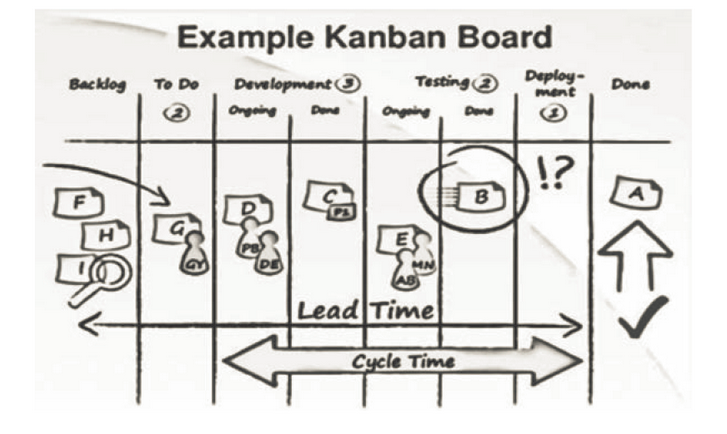
\includegraphics[scale=0.5]{image1.png}
  \caption{Ejemplo de un tablero de Kanban. Extraída de \cite{montegalianoImplantarScrumCon2016}}
  \label{fig:x Tablero kanban}
\end{figure}
\par Las tareas son representadas por tarjetas que avanzan por el tablero a medida que se actualiza su estado actual \cite{montegalianoImplantarScrumCon2016,canosaferreiroSCRUMTeoriaImplementacion2024}. El tablero de trabajo suele tener las siguientes columnas:
\begin{itemize}
    \item \textbf{TO DO}, que representa el trabajo que aún no se ha comenzado.
    \item \textbf{DOING}, que representa el trabajo que se está realizando actualmente.
    \item \textbf{DONE}, que representa el trabajo que se ha completado.
\end{itemize}
\par Este modelo establece una serie de prácticas a seguir:
\begin{itemize}
    \item \textbf{Flujo de trabajo visible}: Las tareas a realizar y el estado en que están son visibles para todos los participantes. Se puede implementar de forma física, utilizando una pared / pizarrón y post-its, o utilizar herramientas como Trello \cite{CaptureOrganizeTackle}. Aún así, es importante plasmar el sistema de forma visual \cite{montegalianoImplantarScrumCon2016,canosaferreiroSCRUMTeoriaImplementacion2024}.
    \item \textbf{Número limitado de tareas}: Para fomentar la agilidad, se limita la cantidad de tareas a realizar. Un miembro del equipo debería tener asignado un número pequeño de tareas en cada columna, de forma que pueda avanzar constantemente. En una situación ideal, un participante es capaz de terminar 1 o 2 tareas al día \cite{montegalianoImplantarScrumCon2016,canosaferreiroSCRUMTeoriaImplementacion2024}.
    \item \textbf{Medir el tiempo de trabajo}: Es importante hacer un seguimiento del avance de las tareas. Recopilar estas métricas permite mejorar los procesos de trabajo y abordar las posibles dificultades que aparezcan  \cite{montegalianoImplantarScrumCon2016,canosaferreiroSCRUMTeoriaImplementacion2024}. Algunas métricas comunes son “lead time”, “touch time” o velocidad, las cuales se estudian en otra sección del trabajo. 
    \item \textbf{Implementar políticas de procesos}: Es necesario establecer criterios que ayuden a mantener un buen ambiente de desarrollo \cite{canosaferreiroSCRUMTeoriaImplementacion2024}. Algunos de ellos pueden ser límite de tareas por personas o protocolos para decidir si una tarea puede ser cancelada o pospuesta. 
\end{itemize}
